\documentclass[Main]{subfiles}
\begin{document}
\FloatBarrier

The planning problem was approached from two different angles, that were intended to be merged later. The two approaches were partial order planning and hierarchical task network. "[!Ref:]" 


\subsubsection{Back tracking}

\textbf{Experimenting with back-tracking}

It was attempted to implement a back-tracking algorithm ....

\todo{Emil}





\subsection{HTN}
As part of the development, a simple HTN algorithm for solving single agent levels were implemented.
The algorithm utilized a genetic algorithm to calculate an optimal order in which to solve the goals.
The motivation for using a genetic algorithm, is that the problem of finding an optimal route to move a set of boxes to a set of goals, can be seen as a traveling salesman problem which is an np-complete task that genetic algorithms can help generate a solution for.
Genetic algorithms cannot calculate the most optimal order, but it can come up with a relative good suboptimal solution in a timely manner. The genetic algorithm used for the HTN experiments is inspired by the implementation at \cite{genetic}.

The genetic algorithm basically works by creating a population which is a list of lists where the inner lists are random permutations of all goals to be completed.
Next the outer list is sorted using an evaluation function which calculates the travel time to complete a given permutation of goals.
The algorithm now mutates and shuffles some of the population by using parts from the best performing permutations.
This goes on until the algorithm doesn't seem to produce good results anymore.

The HTN implementation itself, works by taking set of goals as input, where each goal can be seen as a high level \textit{complex action}. The first goal is chosen and the algorithm decomposes it into a complex action to "move to the box" and a \textit{complex action} to "move the box to the goal". Next the algorithm decomposes the action "move to the box" into primitive actions where only move actions are considered, and the "move box to goal" action into \textit{primitive actions} where all actions are considered.
The algorithm uses the $A^*$ algorithm to decompose into the \textit{primitive actions}.

When the algorithm starts, it only takes the first box for the first goal into account and the rest act as obstacles. When a goal has been completed, the current box remains visible and no longer acts as an obstacle, and can thus still be manipulated. This reduces the branching factor when solving the individual goals in the beginning, -but adds more and more branching factor towards the completion of the unified plan.

The algorithm starts out with a relaxed search space, as it only takes the first box, to be moved to the first goal, into account and deals with the rest of the boxes as obstacles -when solving for the first goal.
When a goal has been completed, the current box remains active and no longer acts as an obstacle so it can be manipulated in the process of solving the next complex actions for the other goals.
This reduces the branching factor when solving the individual goals in the beginning, but adds more and more branching factor towards the completion of the unified plan.

The HTN algorithm is inspired by \cite{nau2003shop2}, where \textit{Tasks} correspond to the highest level complex actions, \textit{Methods} corresponds to decomposition of the top level complex action, \textit{Operators} correspond to \textit{primitive actions} which is derived when refining the \textit{complex actions}, and the \textit{External function call} corresponds to the utilization of the genetic algorithm for finding an optimal goal order.

In the end, the HTN algorithm was discarded because the POP algorithm was performing a lot better and it was therefore chosen to focus on the POP algorithm.


\subsection{General}


\textbf{Experimenting with heuristics}

- Weighted heuristics to encourage specific moves

The heuristics for the full problem search is a simple heuristic calculating the Manhattan distance between the active elements of a node. The active elements being an agent, a goal and a box chosen to solve the goal with. 




\textbf{Experiments with search strategy}


% - Multi vs. single BFS: Should show something about speed versus better solution 

The most interesting experiments conducted with the used search strategy involved two strategies. Best-first search using $A^*$ evaluation and a modified version, multi-queue best-first search using $A^*$ evaluation. The strategy applies to both relaxed and full problem search. 
The multi-queue best-first search utilizes two queues, one active ``main queue'' and one ``back-up queue''. The strategy is a very naive implementation of a multi-queue BFS, as a normal implementation alternates between expansions of the nodes in both queues \citep{hector2013a}, whereas our implementation relies heavily on the ``main queue'' being the \textit{``correct queue''}. Every time a node is expanded, all other nodes in the ``main queue'' are added to the ``back-up queue'' and removed from the main, such that the child nodes from the expanded node are the only nodes in the ``main queue''. In effect this means that our strategy always believes it makes the right choice, which of course is not the case. In the case where the expanded nodes do not lead to solving a goal, the ``main queue'' will at some point turn up empty. When this happens, the most promising node from the ``back-up queue'' is expanded. As the strategy uses $A^*$ evaluation, it is likely that the most promising node will be a node early in the node tree, as its traveled path is short or non-existing. 

The two strategies are compared by comparing the solutions they find to a level. The comparison is regarded from two aspects; completion time, and used actions. As the multi-queue BFS implementation functions as a combination of best-first-search and depth-first-search, it could possibly reach a goal state faster than the normal BFS. The found solution could however be much less than optimal. The standard BFS $A^*$ search is more likely to produce a solution that is more optimal than multi-queue BFS, whereas it might spend more time reaching the goal state. 

As an example of a fast, but ``stupid'' solution solution found using the multi-queue BFS strategy, the level SAHoldkaeft is regarded. A solution to the level is found in 1.6 seconds, with an action set consisting of 536 moves. 

\begin{table}[h]
\begin{tabular}{lll}
\rowcolor{grayish}
\textbf{Strategy} & \textbf{Time} & \textbf{Solution length} \\   %& \textbf{Nodes explored} \\
BFS             & 1.6 s        & 19                       \\    %& 78                      \\
Multi-queue BFS & 22.6 s       & 27                       %& 44                      \\
\end{tabular}
\end{table}

% The single-queue BFS strategy uses 22.6 seconds to find a solution. The solution is however much shorter at 210 moves. 


% Multi-queue BFS:
% Time: 1603 ms
% Actions: 536

% Single-queue BFS:
% Time: 22642 ms
% Actions: 210


\begin{enumerate}
    \item BFS 
    \item Multi-queue BFS (Maybe IDA* or Iterative deepening search)
\end{enumerate}



Benchmarking the multi queue BFS against standard BFS:





\subsection{Preprocessing ----- "??????" }

Experimenting with preprocessing and ``All goals shortest path'' 
- Part of the POP algorithm

- POP run after each solved goal 
--> Better solution --> SO much slower


During development experiments with different strategies regarding preprocessing, or extra-processing providing extra information, were conducted. 

As for the goal ordering based on a relaxed problem search on the initial state, the information about the level at this state is very useful. It is, however, preferred to have the same updated information after each solved goal. The moving of one or more boxes, and the change of the agent's location, will most likely leave the goal sorting less than optimal. It could therefore be beneficial to update the goal sorting, and maybe even the choosing of boxes for goals. 

In order to update the information a relaxed problem search is done based on the state after each goal is solved. 


- Performance affected by number of goals and agents in level, if few, maybe beneficial, if many it could produce a lot of overhead.





\subsection{Benchmark}

All tests and benchmarks found in this paper, as well as the submitted competition results have been performed on computer with the following specifications:

\begin{itemize}
\item CPU: 2.3 GHz Intel Core i7 (I7-4850HQ) 
\item RAM: 8GB dedicated to the JVM
\end{itemize}

\textbf{Frontier testing}

As the search is being done, nodes are being added to the frontier. Before a node is added, a check is performed to see if the node already is in the frontier. As the frontier grows large, this check can be expensive to perform. In order to make the lookup faster, experiments were conducted with a queue and a hash set in parallel. The hash set provides information about whether or not a node is already contained in the frontier.



% % % % % % % % % % % % Something






%%%%%%%%%%%%% Move below to queue experimenting
% 20 second run 
% BFS:
% [Client said] Search starting with strategy Best-first Search (PriorityQueue) using A* evaluation
% [Client said] #Explored:    0, #Frontier:   1, Time: 0.00 s     [Used: 291.41 MB, Free: 316.59 MB, Alloc: 608.00 MB, MaxAlloc: 7282.00 MB]
% [Client said] #Explored: 79000, #Frontier: 11774, Time: 20.33 s     [Used: 893.79 MB, Free: 727.21 MB, Alloc: 1621.00 MB, MaxAlloc: 7282.00 MB]

% Multi queue BFS:
% [Client said] Search starting with strategy Multi-Best-first Search (PriorityQueue) using A* evaluation
% [Client said] #Explored:    0, #Frontier:   1, Time: 0.00 s     [Used: 260.84 MB, Free: 219.66 MB, Alloc: 480.50 MB, MaxAlloc: 7282.00 MB]
% [Client said] #Explored: 256978, #Frontier: 198642, Time: 20.47 s   [Used: 4007.45 MB, Free: 1369.05 MB, Alloc: 5376.50 MB, MaxAlloc: 7282.00 MB]



% From the results it is very clear that the multi queue BFS memory consumption is a great deal higher than single-queue BFS. 



\subsection{Results}
\FloatBarrier

\begin{figure}[h!]
    \centering
    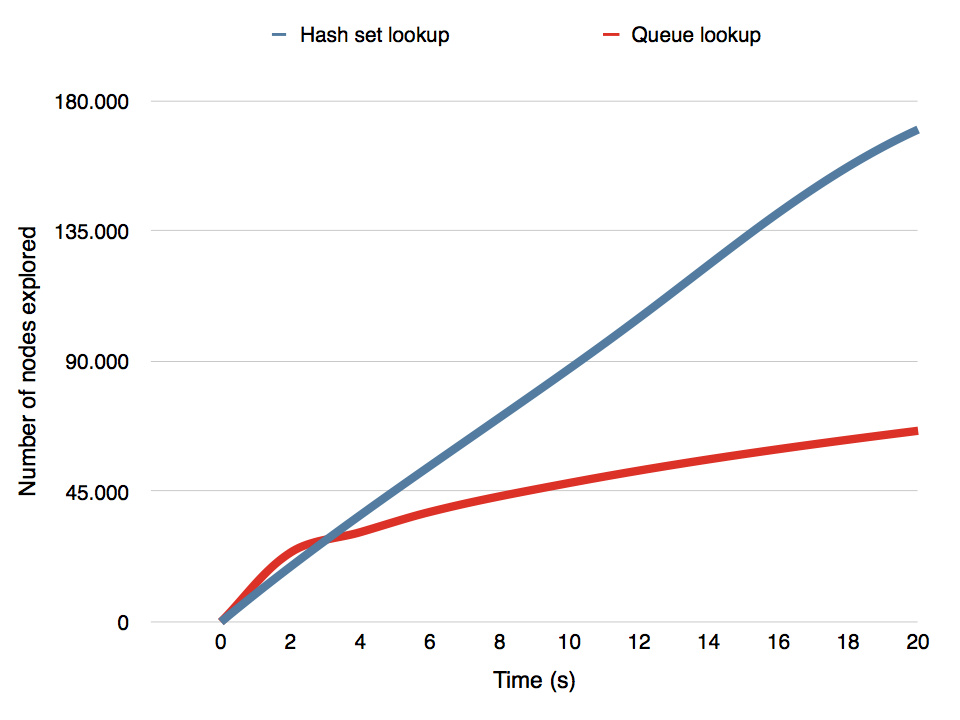
\includegraphics[width=0.5\textwidth]{nodes_explored_compare.png}
    \caption{Comparison of number of nodes explored}
    \label{fig:node_explored_comparison}
\end{figure}

% \begin{figure}[h!]
%     \centering
%     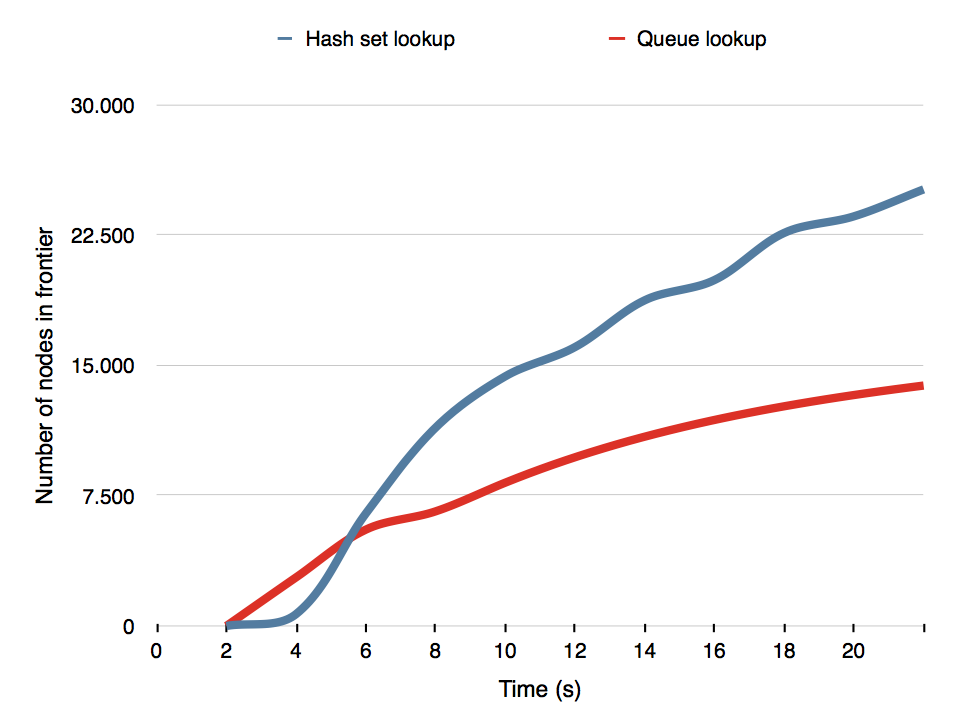
\includegraphics[width=0.3\textwidth]{nodes_in_frontier_compare.png}
%     \caption{Comparison of number of nodes in frontier}
%     \label{fig:node_frontier_comparison}
% \end{figure}

On \autoref{fig:node_explored_comparison} we see a comparison of the performance, between the use of two different data structures for holding nodes. 
The difference is mainly caused by the different performance characteristics for random look ups, 
where a hash set performs look ups in constant time ($O(1)$) in the average case,
priority queues does so linearly to the number of elements in the queue ($O(n)$).

As look ups happen when checking if a node is already explored, the operation happens with a very high frequency, which causes the major difference in performance observed on \autoref{fig:node_explored_comparison}.

\FloatBarrier
\end{document}